% @Author: luis
% @Date:   2016-03-30 22:54:01
% @Last Modified by:   luis
% @Last Modified time: 2016-04-20 12:24:28

\documentclass[12pt]{article}
\usepackage{latexsym}
\usepackage{fancyhdr}
\usepackage{amssymb,amsmath,amsthm}
\usepackage[pdftex]{graphicx}
\usepackage{pdfpages}
\usepackage{hyperref}
\usepackage[margin=1in]{geometry}


% Create answer counter to keep track of seperate responses
\newcounter{AnswerCounter}
\newcounter{SubAnswerCounter}
\newcounter{SubSubAnswerCounter}
\setcounter{AnswerCounter}{1}
\setcounter{SubAnswerCounter}{1}
\setcounter{SubSubAnswerCounter}{1}

% Create answer environment which uses counter
\newenvironment{answer}[0]{
  \setcounter{SubAnswerCounter}{1}
  \bigskip
  \textbf{Solution \arabic{AnswerCounter}}
  \\
  \begin{small}
}{
  \end{small}
  \stepcounter{AnswerCounter}
}

\newenvironment{subanswer}[0]{
  \setcounter{SubSubAnswerCounter}{1}
  (\alph{SubAnswerCounter})
}{
 \bigskip
  \stepcounter{SubAnswerCounter}
}

\newenvironment{subsubanswer}[0]{
  \hspace{0.25in}[\roman{SubSubAnswerCounter}]
}{
 \bigskip
  \stepcounter{SubSubAnswerCounter}
}

% Allows easy use of vectors
\newcommand{\vect}[1]{\boldsymbol{#1}}
\newcommand{\deln}[3]{\frac{\partial^{#3} #1}{\partial #2^{#3}}}
\newcommand{\del}[2]{\frac{\partial#1}{\partial #2}}
\newcommand{\bra}[1]{\langle {#1} |}
\newcommand{\ket}[1]{| {#1} \rangle}
\newcommand{\dt}[2]{\langle {#1} | {#2} \rangle}
\newcommand{\braket}[3]{\langle {#1} | {#2} | {#3} \rangle}
\newcommand{\op}[1]{{#1}_{op}}
\newcommand{\opb}[1]{{\bf {#1}}_{op}}


% Custom Header information on each page
\pagestyle{fancy}
\lhead{HUID: 70871564}
\rhead{Luis Perez - \thepage}
\renewcommand{\headrulewidth}{0.1pt}
\renewcommand{\footrulewidth}{0.1pt}

\newcommand{\horrule}[1]{\rule{\linewidth}{#1}}   % Horizontal rule
\title{
    % \vspace{-1in}
    \usefont{OT1}{bch}{b}{n}
    \normalfont \normalsize \textsc{Harvard University} \\ [25pt]
    \horrule{0.5pt} \\[0.4cm]
    \huge Physics 143a: Quantum Mechanics I \\ [20pt]
    \normalfont \normalsize Problem Set 7
    \horrule{2pt} \\[0.5cm]
}
\author{
    \normalfont                 \normalsize
        Luis Antonio Perez\\[-3pt]    \normalsize
}
\date{\today}

\begin{document}
\maketitle
\pagebreak

\begin{answer}
In this question we consider the rotation operator which rotates a system by an angle $\alpha$ about the $\hat{n}$ direction. The operator is given by:
$$
R_{\hat{n}}(\alpha) = \exp \frac{-i\alpha \hat{L} \cdot \hat{n}}{\hbar}
$$

\begin{subanswer}
We calculate the operator for an infinitesimal rotation.
$$
R_{\hat{n}}(d\alpha) = \exp \frac{-i(d\alpha) \hat{L} \cdot \hat{n}}{\hbar} = \sum_{k=0}^{\infty} \frac{(-i(d\alpha)\hat{L}\cdot\hat{n})^k}{k!} \approx I - \frac{i(d\alpha)}{\hbar}\hat{L} \cdot \hat{n}
$$
because given that $d\alpha \to 0$, we can ignore terms with exponent larger than $1$.
\end{subanswer}

\begin{subanswer}
We recall that the states described by $l,m$ (spherical harmonics) are given by the below, where we've left out the dependence on $r$ as we know that rotations maintain distances:
$$
Y_{l,m}(\theta, \phi) = c(l,|m|)e^{im\phi}P_{l,m}(\cos\theta)
$$
where $c(\cdot,\cdot)$ is simply the normalization constant. If we consider a rotation by $\phi_0$ about the $z$-axis, we'll have the following:
\begin{align*}
R_{\hat{z}}(\phi_0)Y_{l,m}(\theta, \phi) &= c(l,|m|)e^{im\phi}P_{l,m}(\cos\theta) \tag{focus only on the term dependent on $\phi$}\\
&= e^{\frac{-i \phi_0 L_z}{\hbar}} e^{im\phi} c(l, |m|)P_{l,m}(\cos\theta) \\
&= e^{-\phi_0\del{}{\phi}} e^{im\phi} c(l, |m|)P_{l,m}(\cos\theta) \tag{recall $L_z = -i\hbar\del{}{\phi}$}\\
&= \sum_{k=0}^{\infty} \frac{(-\phi_0)^k}{k!} \deln{}{\phi}{k}e^{im\phi} c(l, |m|)P_{l,m}(\cos\theta) \\
&= \sum_{k=0}^{\infty} \frac{(-\phi_0)^k}{k!} (im)^k e^{im\phi} \\
&= e^{-i\phi_0m}e^{im\phi} c(l, |m|)P_{l,m}(\cos\theta) \\
&= e^{im(\phi - \phi_0)} c(l, |m|)P_{l,m}(\cos\theta) \\
&= Y_{l,m}(\theta, \phi - \phi_0) \tag{we use the fact that nothing else has changed}
\end{align*}
This matches our intuition as to what the final result should be, which is simply a rotation by $\phi_0$ about the positive $z$-axis.

Note that any state with $m = 0$ does not have access to the rotations in the sense that a rotation will leave the exponent untouched.
\end{subanswer}

\begin{subanswer}
We can show this explicitly using the above results with $\phi_0 = \pi$ (we transform to radians).
\begin{align*}
  R_{\hat{z}}(\pi)Y_{l,m}(\theta, \phi) &= e^{im(\phi - \pi)} c(l, |m|)P_{l,m}(\cos\theta) \\
  &= e^{-im\pi}e^{im\phi} c(l, |m|)P_{l,m}(\cos\theta) \\
  &= (-1)^mY_{l,m}(\theta, \phi)
\end{align*}
\end{subanswer}

\begin{subanswer}
We present the more involved algebraic solutions which simply involves a lot of simplifications steps. We attempt to be as clear as possible in the results. Recall the following facts:
\begin{align*}
L_x &= i\hbar \left[\sin \phi \del{}{\theta} + \cot \theta \cos \phi \del{}{\phi} \right] \\
L_y &= i\hbar\left[-\cos \phi \del{}{\theta} + \cot \theta \sin \phi \del{}{\phi}\right] \\
L_z &= -i\hbar \del{}{\phi} \\
L^2 &= -\hbar^2\left[\frac{1}{\sin \theta}\del{}{\theta}\left(\sin \theta \del{}{\theta} \right) + \frac{1}{\sin^2 \theta} \deln{}{\theta}{2} \right]
\end{align*}
We begin by first simplifying the raising operator:
\begin{align*}
L_+ &= L_x + iL_y \\
&= i\hbar \left[\sin \phi \del{}{\theta} + \cot \theta \cos \phi \del{}{\phi} \right] - \hbar\left[-\cos \phi \del{}{\theta} + \cot \theta \sin \phi \del{}{\phi}\right] \\
&= \hbar \left[(\cos \phi + i \sin \phi)\del{}{\theta} + i(\cos\phi + i\sin \phi )\cot \theta \del{}{\phi} \right] \\
&= \hbar e^{i\phi}\left[\del{}{\theta} + i\cot \theta \del{}{\phi} \right]
\end{align*}
and similarly for the lowering operator:
\begin{align*}
L_- &= L_x - iL_y \\
&= i\hbar \left[\sin \phi \del{}{\theta} + \cot \theta \cos \phi \del{}{\phi} \right] + \hbar\left[-\cos \phi \del{}{\theta} + \cot \theta \sin \phi \del{}{\phi}\right] \\
&= \hbar \left[-(\cos \phi - i \sin \phi)\del{}{\theta} + i(\cos\phi - i\sin \phi )\cot \theta \del{}{\phi} \right] \\
&= \hbar e^{-i\phi}\left[-\del{}{\theta} + i\cot \theta \del{}{\phi} \right]
\end{align*}
and note that the lowering and raising operators are adjoints of each other. In the sense that:
$$
L_+^\dag = L_-, \quad L_-^\dag = L_+
$$
Now we can compute the result we're looking for. We do it for the raising operator first:
\begin{align*}
L_+^\dag L_+ &= L_-L_+ \\
&=  \hbar e^{-i\phi}\left[-\del{}{\theta} + i\cot \theta \del{}{\phi} \right] \left( \hbar e^{i\phi}\left[\del{}{\theta} + i\cot \theta \del{}{\phi} \right]\right) \\
&= \hbar e^{-i\phi} \left[ -\del{}{\theta}\left( \hbar e^{i\phi}\left[\del{}{\theta} + i\cot \theta \del{}{\phi} \right]\right) + i\cot \theta \del{}{\phi} \left( \hbar e^{i\phi}\left[\del{}{\theta} + i\cot \theta \del{}{\phi} \right]\right) \right] \\
&= \hbar e^{-i\phi} \left[-\hbar e^{i\phi} \deln{}{\theta}{2} + i \frac{1}{\sin^2 \theta}\del{}{\phi} + i \cot \theta \del{}{\theta} \del{}{\phi} + \phi \cot \theta \del{}{\theta} - i\cot \theta \del{}{\phi}\del{}{\theta} + i\phi \cot^2 \theta \del{}{\phi} + \cot^2 \theta \deln{}{\phi}{2}\right] \\
&= -\hbar^2 \left[\deln{}{\theta}{2} + \cot \theta \del{}{\theta} + \frac{1}{\sin^2 \theta} \deln{}{\phi}{2} - \deln{}{\phi}{2} - i \del{}{\phi} \right] \tag{assuming nice w.f.} \\
&= -\hbar^2 \left[\deln{}{\theta}{2} + \cot \theta \del{}{\theta} + \frac{1}{\sin^2 \theta} \deln{}{\phi}{2} \right] + \hbar^2 \deln{}{\phi}{2} + i\hbar^2\del{}{\phi} \\
&= L^2 - L_z^2 - \hbar L_z
\end{align*}
and we repeat the process for the down lowering operator:
\begin{align*}
L_-^\dag L_- &= L_+L_- \\
&=  \hbar e^{i\phi}\left[\del{}{\theta} + i\cot \theta \del{}{\phi} \right] \left( \hbar e^{-i\phi}\left[\del{}{\theta} + i\cot \theta \del{}{\phi} \right]\right) \\
&= \hbar e^{i\phi} \left[ \del{}{\theta}\left( \hbar e^{-i\phi}\left[\del{}{\theta} + i\cot \theta \del{}{\phi} \right]\right) + i\cot \theta \del{}{\phi} \left( \hbar e^{-i\phi}\left[\del{}{\theta} + i\cot \theta \del{}{\phi} \right]\right) \right] \\
&= \hbar e^{i\phi} \left[-\hbar e^{-i\phi} \deln{}{\theta}{2} + i \frac{1}{\sin^2 \theta}\del{}{\phi} + i \cot \theta \del{}{\theta} \del{}{\phi} + \phi \cot \theta \del{}{\theta} - i\cot \theta \del{}{\phi}\del{}{\theta} + i\phi \cot^2 \theta \del{}{\phi} + \cot^2 \theta \deln{}{\phi}{2}\right] \\
&= -\hbar^2 \left[\deln{}{\theta}{2} + \cot \theta \del{}{\theta} + \frac{1}{\sin^2 \theta} \deln{}{\phi}{2} - \deln{}{\phi}{2} - i \del{}{\phi} \right] \tag{assuming nice w.f.} \\
&= -\hbar^2 \left[\deln{}{\theta}{2} + \cot \theta \del{}{\theta} + \frac{1}{\sin^2 \theta} \deln{}{\phi}{2} \right] + \hbar^2 \deln{}{\phi}{2} + i\hbar^2\del{}{\phi} \\
&= L^2 - L_z^2 - \hbar L_z
\end{align*}
\end{subanswer}

\begin{subanswer}
Using commutators we have the following result:
\begin{align*}
  L_{\pm}^\dag L_{\pm} &= (L_x \pm iL_y)^{\dag}(L_x \pm iL_Y) \tag{definition }\\
  &= (L_x \mp iL_y)(L_x \pm iL_Y) \tag{Each $L_i$ is Hermitian.} \\
  &= L_x^2 + L_y^2 \pm iL_xL_y \mp iL_xL_y \\
  &= L^2 - L_z^2 \pm i[L_x, L_y] \\
  &= L^2 - L_z^2 \pm i(i\hbar L_z) \\
  &= L^2 - L_z^2 \mp \hbar L_z
\end{align*}
and we are done, as desired.
\end{subanswer}
\end{answer}

\begin{answer}
We now focus on the hydrogen atom/ion and solve the quantum mechanical system corresponding to it. We follow the treatment presented in Griffith:

\begin{subanswer}
The potential for the atom/ion is given by:
$$
V(r) = -\frac{e^2}{4\pi \epsilon_0} \frac{Z}{r}
$$
and plugging into the radial equations we have:
$$
-\frac{\hbar^2}{2m}\deln{u}{r}{2} + \left[-\frac{e^2}{4\pi \epsilon_0} \frac{Z}{r} +\frac{\hbar^2}{2m}\frac{l(l+1)}{r^2} \right]u = Eu
$$
where we've defined $u(r) = rR(r)$ with the additional restriction that as $r \to 0$, we must have that $u(r) \to 0$. Note that the coordinate system is nucleus-centric so we can avoid having to deal with total operators and total ass.
We focus only on the discrete bound states. To make notation easier, define:
$$
k \equiv \frac{\sqrt{-2mE}}{\hbar}
$$
where $k$ is real since for bound states (which are the ones we care about) we have $E < 0$. We also define:
$$
\rho \equiv k r, \quad \rho_0 \equiv \frac{Zme^2}{2\pi\epsilon_0\hbar^2 k}
$$
then taking the TISE and diving by $E$, rearranging, and using our defined constants:
\begin{align*}
-\frac{\hbar^2}{2mE}\deln{u}{r}{2} + \left[-\frac{e^2}{4\pi \epsilon_0 E} \frac{Z}{r} +\frac{\hbar^2}{2m E}\frac{l(l+1)}{r^2} \right]u = u \\
\implies \frac{1}{k^2}\deln{u}{r}{2} = \left[1 + \frac{l(l+1)}{(kr)^2} - \frac{me^2}{2\pi \epsilon_0\hbar^2k}\frac{Z}{kr} \right]u \\
\implies \deln{u}{\rho}{2} = \left[1 + \frac{l(l+1)}{\rho^2} - \frac{\rho_0}{\rho} \right]u
\end{align*}
If we example the case as $r \to \infty \implies \rho \to \infty$, we see that we have the following approximation:
$$
\deln{u}{\rho}{2} = u
$$
which for reasons discussed before has the admissible solution:
$$
u(\rho) \approx Ae^{-\rho}
$$
and for small $\rho \to 0$ (as long as $l \neq 0$) we have:
$$
\deln{u}{\rho}{2} = \frac{l(l+1)}{\rho^2}u
$$
which has general solutions:
$$
u(\rho) = C\rho^{l+1} + D\rho^{-l}
$$
where we must have $D = 0$ to have an admissible solution. Therefore:
$$
u(\rho) \approx C\rho^{l+1}
$$
for $\rho \to 0$. As in Griffith, we introduce the new function $v(\rho)$ to capture the non-asymtotic behaviour of $u$. We have:
$$
u(\rho) = e^{-\rho}\rho^{l+1}v(\rho)
$$
which gives us:
$$
\del{u}{\rho} = \rho^{l}e^{-\rho}[(l+1 - \rho)v + p \del{v}{p}]
$$
and therefore:
$$
\deln{u}{\rho}{2} = \rho^{l}e^{-\rho}\left\{\left[-2l + 2 + \rho + \frac{l(l+1)}{\rho} \right]v + 2(l+1 - \rho)\del{v}{\rho} + \rho \deln{v}{\rho}{2}\right\}
$$
Then with a bit of algebra we can rewrite the radial equation in terms of $v$ as:
$$
\rho \deln{v}{\rho}{2} + 2(l+1 - \rho)\del{v}{\rho} + [\rho_0 - 2(l+1)]v = 0
$$
Now we make the assumption that the solution $v$ can be expressed as a power series.
$$
v(\rho) = \sum_{k=0}^{\infty} c_j \rho^j
$$
where
$$
\del{v}{\rho} = \sum_{j=0}^{\infty} (j+1)c_{j+1}\rho^{j}
$$
and
$$
\deln{v}{\rho}{2} = \sum_{j=1}^{\infty} j(j+1)c_{j+1}\rho^{j-1}
$$
If we insert the above into the radial equation and then equate the resulting polynomial to the zero poylnomial, which occurs iff all coefficients with matching powers of $\rho$ matches, we arrive that the following recursive relations among the coefficeints:
$$
c_{j+1} = \frac{2(j+l +1) - \rho_0}{(j+1)(j + 2l + 2)}
$$
Note that the only way to prevent a blow-up in the equations is to have the series above terminate for some coefficient, in the sense that if it terminates at $c_k$, then this implies that $\forall i > k$, $c_i = 0$. We must therefore have that $2(j+l +1) - \rho_0 = 0$ so we define the qunatum number $n \equiv j_{max} + l + 1$. We therefore have the restrictions that:
$$
\rho_0 = 2n
$$
and plugging in our definition of $\rho_0$ and solving for $k$, we get:
$$
k = \frac{Zme^2}{4\pi \epsilon_0 \hbar^2}\frac{1}{n}
$$
Therefore recalling that the energies are given by:
$$
E_n = -\frac{\hbar^2 k^2}{2m} = -\frac{Z^2me^4}{32 \pi^2\epsilon_0^2\hbar^2} = - \left[\frac{m}{2\hbar^2}\left(\frac{Ze^2}{4\pi\epsilon_0} \right)^2 \right]\frac{1}{n^2} = -\frac{E_1}{n^2}
$$
for $n = 1,2,3,\cdots$ which gives the quantized energy levels for the hydrogen atom! Woop! :) Note that we can plug in the constants an obtain, where we also take $Z = 1$ (for the hydrogen atom):
$$
E_1 = 13.6 eV
$$
which we use from this point forward.
\end{subanswer}

\begin{subanswer}
The energy levels indirectly depend on the quantum numbers $l,m$ because we defined:
$$
n \equiv j_{max} + l + 1 \implies j_{max} = n - l - 1
$$
and we know $j_{max} \geq 0$. Therefore, given a fixed value for $n$, we must have that $l = 0,1,\cdots,n-1$ in order for this property to be satisfied. Then we know from the spherical harmonics that $|m| < l$. Note that all of these states have the exact same energy, since the energy depends exclusively on $n$.
\end{subanswer}

\begin{subanswer}
The number of degenerate states is easy to derive. Given a fixed value for $n$, we have $2l + 1$ states per each possible value of $l$, of which there are $n$. This gives:
$$
\sum_{l=0}^{n-1} 2l + 1 = n^2
$$
since it is the sum of the first $n$ odd values. The above is the degeneracy of the state with energy $E_n$.
\end{subanswer}

\begin{subanswer}
We can natural derive the Bohr radius. Recalling our definition of $\rho_0$ and comparing it to the Bohr radius $a_0$:
\begin{align*}
\rho_0 &\equiv \frac{Zme^2}{2\pi\epsilon_0\hbar^2 k}, \quad \rho_0 = 2n \\
\implies& k = \left(\frac{Zme^2}{4\pi\epsilon_0\hbar^2} \right)\frac{1}{n} = \frac{1}{a_0} \frac{1}{n}
\end{align*}
which implies a natural choice for the Bohr radius as:
$$
a_0 = \frac{4\pi\epsilon_0\hbar^2}{Zme^2}
$$
where $n$ is playing the role of $Z$.
\end{subanswer}
\end{answer}

\begin{answer}
We now consider specific Hydrogen atoms examples.

\begin{subanswer}
The graphical representation is presented below:
\begin{figure}[h!]
\centering
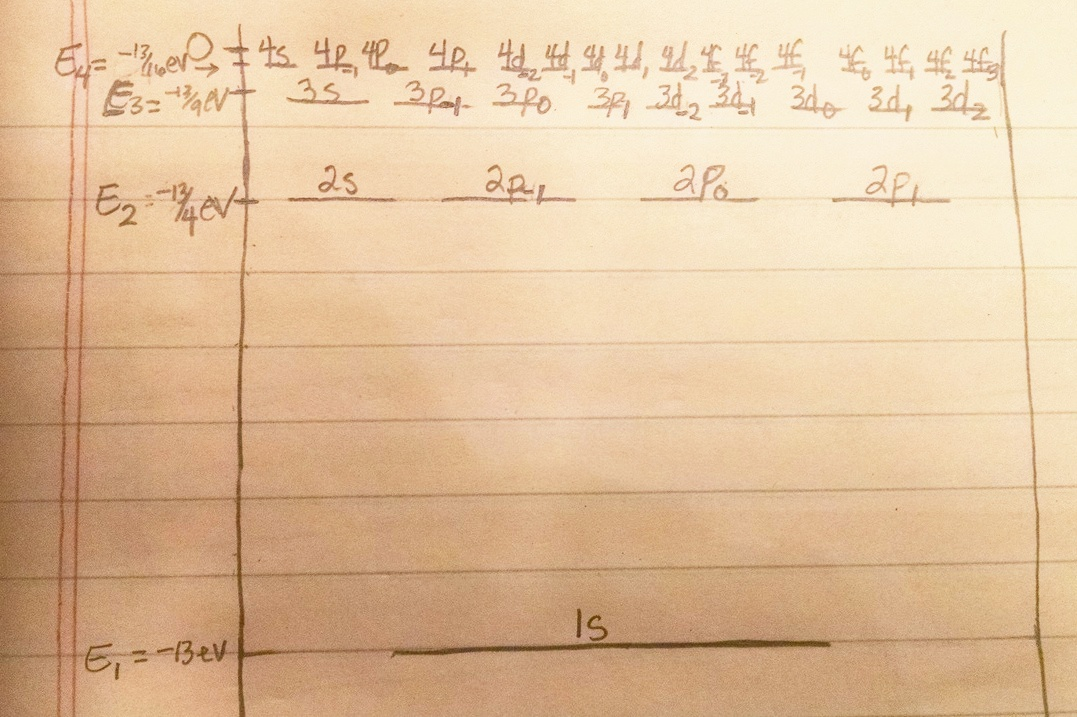
\includegraphics[scale=0.2]{energy-levels.jpg}
\caption{The energy levels for the first four energy eigenstates of the Hydrogen atom/ion model. Note that another page is attached which lets us define the results more clearly because printing is usually of poor quality.}
\label{fig:energy_levels}
\end{figure}
\end{subanswer}

\begin{subanswer}
We derive the frequency of a photon which plays part in the transition of the hydrogen atom from the state $n_i$ to the state $n_f$. Let $E_1$ be defined as before ($\approx 13.6 eV$). Then we have:
$$
E = E_f - E_i = E_1\left(\frac{1}{n_f} - \frac{1}{n_i}\right)
$$
which implies that the frequency is simply:
$$
f = \frac{E_1}{h}\left(\frac{1}{n_f} - \frac{1}{n_i}\right)
$$
and in terms of the Rydberg constant, we have the frequency as:
$$
f = cR_{\infty}\left(\frac{1}{n_f} - \frac{1}{n_i}\right)
$$
since $R_{\infty} = \frac{m}{4\pi c \hbar^4}\left(\frac{e^2}{4\pi\epsilon_0} \right)^2$.
\end{subanswer}

\begin{subanswer}
The Griffith problem is as follows.

\begin{subsubanswer}
The new potential is given by the gravitational potential:
$$
U(r_0) = -GMm\frac{1}{r_0}
$$
where $G$ is the gravitational constants given by $G = 6.673 \times 10^{-11} m^3 kg^{-1} s^{-2}$
\end{subsubanswer}

\begin{subsubanswer}
Recall the the Bohr Radius in general, with potential given by:
$$
V(r_0) = -\alpha \frac{1}{r_0}
$$
is given by:
$$
a = \frac{1}{\alpha} \frac{\hbar^2}{m}
$$
so this gives the Bohr readius for the earth-sun system as:
$$
a = \frac{\hbar^2}{GMm^2}
$$
which we can calculate to be the actual numerical value of:
$$
a = 2.349 \times 10^{-138} m
$$
which is extremely small... (but I double checked!)
\end{subsubanswer}

\begin{subsubanswer}
Recall that for the generalized potential above the energy levels are given by:
$$
E_n = - \left[ \frac{m}{2\hbar^2} \alpha^2 \right] \frac{1}{n^2}
$$
so plugging in $\alpha = GMm$ we have the following energy levels for the earth/sun system:
$$
E_n = - \left[ \frac{m}{2\hbar^2} G^2M^2m^2 \right] \frac{1}{n^2}
$$
The above is the total energy of the system. Classically, we can calculate this total energy in another way, by summing the KE and Potential Energy. For the sun/earth system, we've already given above the potential energy. The kinetic energy is given by equating the centripetal force with the gravitational force:
\begin{align*}
\frac{mv^2}{r_0} &= \frac{GMm}{r_0^2} \\
\implies \frac{1}{2}mv^2 &= \frac{GMm}{2r_0}
\end{align*}
Therefore the total energy is now:
$$
E_T = -GMm(\frac{1}{r_0} - \frac{1}{2r_0}) = -\frac{GMm}{2r_0}
$$
Equating the two and solving for $n$:
\begin{align*}
- \left[ \frac{m}{2\hbar^2}(GMm)^2 \right] \frac{1}{n^2} &= -\frac{GMm}{2r_0} \\
\implies n^2 &= \frac{GMm^2r_0}{\hbar^2} \\
\implies n^2 &= \frac{r_0}{a} \\
\implies n &= \sqrt{\frac{r_0}{a}}
\end{align*}
as desired. We now that $r_0 \approx =1.4598 \times 10^{11} m$, so we have its quantum number as:
$$
n \approx 2.524 \times 10^74
$$
which is hella large.
\end{subsubanswer}

\begin{subsubanswer}
If the Earth made a transition to the next lower energy level, the energy released would be proportional to the following, where we use the general energy level $n$
\begin{align*}
\frac{1}{(n-1)^2} - \frac{1}{n^2} &= \frac{n^2 - (n-1)^2}{[(n-1)n]^2} \\
&= \frac{2n - 1}{(n^2 - n)^2} \\
&\approx \frac{2n}{n^4} \tag{for large $n$} \\
&= \frac{2}{n^3}
\end{align*}
So the energy released will be approximately:
$$
\Delta E = \frac{m(GMm)^2}{2\hbar^2}\frac{2}{n^3} \approx 2.1 \times 10^{-41}J
$$
when we plugin our constants. First, note that the frequency of the photon/graviton is:
$$
v = \frac{\Delta E}{h} = 3.168 \times 10^{-8} s^{-1}
$$
The wavelength of the emitted photon/graviton would be:
\begin{align*}
\lambda &= \frac{c}{v} \\
&= 9.469 \times 10^{15} m
\end{align*}
which is approximately 1 light year.
\end{subsubanswer}
\end{subanswer}
\end{answer}

\begin{answer}
We now tackle the problem of determining the matrices $\boldsymbol{L}$. We make use of the following eigenvalues for the state $\ket{l,m}$. Furthermore, we note that none of the operators have any effect on the $r$ component of our w.f.s, therefore we can simply ignore it. We being with $L^2$. First, recall the general formula, generalized to include the quantum number $n$:
$$
L^2 \ket{n,l,m} = \hbar^2 l(l+1)\ket{n,l,m}
$$
which gives us the following set of equations:
\begin{align*}
L^2 \ket{1,0,0} &= 0 \ket{1,0,0} = 0\\
L^2 \ket{2,1,1} &= 2\hbar^2 \ket{2,1,1} \\
L^2 \ket{2,1,0} &= 2\hbar^2 \ket{2,1,0} \\
L^2 \ket{2,1,-1} &= 2\hbar^2 \ket{2,1,-1}
\end{align*}
Therefore, the matrix is given by:
$$
L^2 = 2\hbar^2\begin{pmatrix}
0 & 0 & 0 & 0 \\
0 & 1 & 0 & 0 \\
0 & 0 & 1 & 0 \\
0 & 0 & 0 & 1 \\
\end{pmatrix}
$$
with the given basis. Now we tackle $L_z$. Recall:
$$
L_z \ket{n,l.m} = \hbar m \ket{n,l.m}
$$
which depends only on $m$ and gives us the following:
\begin{align*}
L_z \ket{1,0,0} &= 0 \ket{1,0,0} = 0\\
L_z \ket{2,1,1} &= \hbar \ket{2,1,1} \\
L_z \ket{2,1,0} &= 0 \ket{2,1,0} = 0 \\
L_z \ket{2,1,-1} &= -\hbar \ket{2,1,-1}
\end{align*}
which we can then put into matrix form as:
$$
L_z = \hbar \begin{pmatrix}
0 & 0 & 0 & 0 \\
0 & 1 & 0 & 0 \\
0 & 0 & 0 & 0 \\
0 & 0 & 0 & -1 \\
\end{pmatrix}
$$
We tackle the raising/lowering operators, which we then use to calculate $L_x$. Note that $L_- = L_+^\dag$, so we really only need to calculate the raising operator. Then we can use the fact that $L_+ + L_+^\dag = 2L_x$ to determine $L_x$. Recall the following generalized statement:
$$
L_+ \ket{n,l.m} = \hbar\sqrt{(l-m)(l+m+1)} \ket{n,l,m+1}
$$
which then gives us the below results:
\begin{align*}
L_+ \ket{1,0,0} &= 0 \ket{1,0,1} = 0\\
L_+ \ket{2,1,1} &= 0 \ket{2,1,2} = 0 \\
L_+ \ket{2,1,0} &= \hbar\sqrt{2} \ket{2,1,1} \\
L_+ \ket{2,1,-1} &= \hbar\sqrt{2} \ket{2,1,0}
\end{align*}
which we can then put into matrix form as:
$$
L_+ = \hbar\sqrt{2} \begin{pmatrix}
0 & 0 & 0 & 0 \\
0 & 0 & 1 & 0 \\
0 & 0 & 0 & 1 \\
0 & 0 & 0 & 0 \\
\end{pmatrix}
$$
and we can immediately calculate:
$$
L_- = L_+^\dag = \hbar\sqrt{2} \begin{pmatrix}
0 & 0 & 0 & 0 \\
0 & 0 & 0 & 0 \\
0 & 1 & 0 & 0 \\
0 & 0 & 1 & 0 \\
\end{pmatrix}
$$
which gives us:
$$
L_x = \frac{\hbar}{\sqrt{2}} \begin{pmatrix}
0 & 0 & 0 & 0 \\
0 & 0 & 1 & 0 \\
0 & 1 & 0 & 1 \\
0 & 0 & 1 & 0 \\
\end{pmatrix}
$$
Note that we can also go ahead and compute $L_y$ by noting that:
$L_+ - L_- = 2iL_y \implies L_y = -\frac{i}{2}L_+ - L_-$ to arrive at:
$$
L_y = \frac{i\hbar}{\sqrt{2}} \begin{pmatrix}
0 & 0 & 0 & 0 \\
0 & 0 & -1 & 0 \\
0 & 1 & 0 & -1 \\
0 & 0 & 1 & 0 \\
\end{pmatrix}
$$
and we are done.
\end{answer}

\begin{answer}
We now tackle the problem of plotting a few values for the hydrogen ion with $Z = 3$:
\begin{subanswer}
We first note that the only change required when $Z = 3$ is given by the Bohr radius. We now have a Bohr radius of:
$$
a = \frac{1}{3}a_0
$$
where $a_0$ is the Bohr radius for the hydrogen atom. This gives us a new value of:
$$
a \approx 1.76 \times 10^{-11} m
$$
This is the value we use when calculating the radial functions. The spherical harmonics remains the same. This is because we have:
$$
\Psi_{nlm}(r,\theta,\phi) = R_{nl}(r)Y_{lm}(\theta,\phi)
$$
so the spherical harmonics do not depend on $r$. We can plot those directly using the function {\sc SphereicalHarmonicsY}. For the radial function, we know that they are given by:
$$
R_{nl}(r) = \frac{1}{r}\rho^{l+1}e^{-\rho}v(\rho)
$$
where $\rho$ is defined by:
$$
\rho = \frac{r}{an}
$$
and the polynomial $v(\rho) = L^{2l + 1}_{n-l-1}(2\rho)$ where $L$ is the associated Laguerre polynomial. We code these directly into our problem statement. For $n = 2, l = 0, m = 0$ we have:
$$
L_1^1(x) = -2x+4
$$
so we have the normalized radial function:
\begin{align*}
R_{20}(r) &= \frac{1}{\sqrt{2}}a^{-3/2}(1 - \frac{r}{2a})e^{-r/(2a)}
\end{align*}
Putting the above together in to Mathematica, we can generate the below plot shown in Figure \ref{fig:200plot}:
\begin{figure}[h!]
\centering
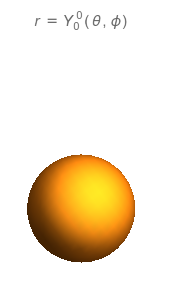
\includegraphics[scale=0.4]{200plot.png}
\caption{Probability density plot of $Y_{200}$}.
\label{fig:200plot}
\end{figure}
\end{subanswer}

\begin{subanswer}
The approach is similar to the above where we modify the radial function and utilized the spherical harmonics functionality of Mathematica to generate our results, as shown in Figure \ref{fig:200plot}.

\begin{figure}[h!]
\centering
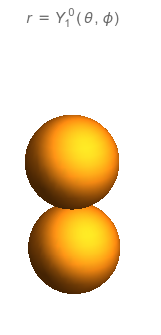
\includegraphics[scale=0.4]{210plot.png}
\caption{Probability density plot of $Y_{210}$}.
\label{fig:200plot}
\end{figure}

We first note that in this case we have:
$$
L^3_1(x) = 6
$$
so we have the normalized result (taken from Griffith):
\begin{align*}
R_{21}(r) &= \frac{1}{r}\rho^2 e^{-\rho}(6) \\
&= \frac{1}{\sqrt{24}}a^{-3/2}\frac{r}{a}e^{-r/(2a)}
\end{align*}

For reference, we also include the plots provided by the textbook, as we can see that our plots match closely. See Figure \ref{fig:bookplots}.

\begin{figure}[h!]
\centering
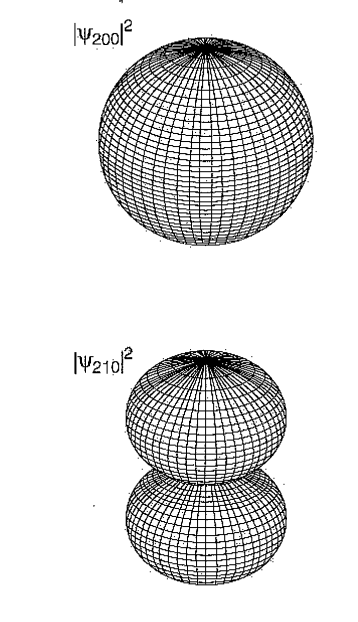
\includegraphics[scale=0.4]{bookplots.png}
\caption{Probability density plot of $Y_{200}$ and $Y_{210}$ as presented in Griffith.}.
\label{fig:bookplots}
\end{figure}

\end{subanswer}

\begin{subanswer}
To calculate $\langle r \rangle$ for the ground state, we need to explicitly know $Y_{00}$. We already have from above the value of $R_{20}$, and we recall that the value for the spherical harmonic is:
$$
Y_{00}(\theta, \phi) = \frac{1}{2\sqrt{\pi}}
$$
so putting everything together:
$$
Y_{200}(r,\theta, \phi) =\frac{1}{2\sqrt{2\pi}}a^{-3/2}(1-\frac{r}{2a})e^{-r/(2a)}
$$
so we calculate the average value directly simply be integrating. Note that the calculation is simplified by the fact that the function only depends on $r$:
\begin{align*}
\langle r \rangle &= \frac{1}{8\pi a^3}\int r^3 (1 - \frac{r}{2a})^2e^{-r/a}  d\Omega dr \\
&= \frac{a}{2} \int_{0}^{\infty} u^3 (1 - u/2)^2 e^{-u} du \\
&= 6a
\end{align*}
\end{subanswer}

\begin{subanswer}
We perform a similar computation to the above:
\begin{align*}
\langle r^2 \rangle &= \frac{1}{8\pi a^3}\int r^4 (1 - \frac{r}{2a})^2e^{-r/a}  d\Omega dr \\
&= \frac{a^2}{2} \int_{0}^{\infty} u^4 (1 - u/2)^2 e^{-u} du \\
&= 42a^2
\end{align*}
\end{subanswer}

\begin{subanswer}
By symmetry of the ground state, we have that $\langle x \rangle = 0$.
\end{subanswer}

\begin{subanswer}
We can use the fact that $r^2 = x^2 + y^2 + z^2$. By symmetry, because for the ground state the axis are interchangeable, we must have that:
$$
\langle x^2 \rangle = \langle y^2 \rangle  = \langle z^2 \rangle  = \langle r^2 \rangle / 3 = 14a
$$
\end{subanswer}

\begin{subanswer}
The most probable value of $r$ is given when we find the maximum with respect to $r$ of $|Y_{200}|^2$. Note that this is equivalent to finding the maximum of $|R_{20}|^2$. The function is simply $\frac{1}{2a^3}(1-r/(2a))^2e^{-r/2a}$. Taking the derivative and setting equal to zero, we arrive at the following equation:
\begin{align*}
-\frac{1}{4a^4}(1 - r/(2a))e^{-r/(2a)} - \frac{1}{4a^4}(1-r/(2a))^2e^{-r/(2a)} &= 0 \\
\implies (1-r/(2a))[1 - (1-r/(2a))] &= 0 \\
\implies r = 2a, \quad r=4a
\end{align*}
So it turns out that we actually have two peaks for the probability. It's interesting to note that this occurs, given how the system is structured.
\end{subanswer}

\begin{subanswer}
We can now as we did before. Note that we cannot take advantage of symmetry this time around because the system is not symmetric about all three axis. However, we can directly calculate the results just as before:
$$
Y_{21-1}(r,\theta, \phi) = R_{21}(r)Y_{1-1}(\theta, \phi) = \sqrt{\frac{3}{8(24)\pi}}a^{-3/2}\frac{r}{a}\sin \theta e^{-i\phi-r/(2a)}
$$
Then calculating the integral using the identity that $x = r \sin \theta \cos \phi$:
\begin{align*}
\braket{Y_{21-1}}{r \sin \theta \sin \phi}{Y_{21-1}} &= \frac{3}{8\pi}\frac{1}{24a^5} \int_0^{2\pi} \cos^2 \phi d\phi \int_0^{\pi} \sin^5 \theta d\theta \int_0^{\infty} r^6 e^{-r/a} dr \\
&=  \frac{1}{2}  \frac{3}{8\pi}\frac{1}{24a^5}\int_0^{2\pi} \cos 2\phi + 1 d\phi \int_0^{\pi} \sin^5 \theta d\theta \int_0^{\infty} r^6 e^{-r/a} dr \\
&=  \frac{3}{8}\frac{1}{24a^5}\int_0^{\pi} \sin^5 \theta d\theta \int_0^{\infty} r^6 e^{-r/a} dr \\
&= \frac{3}{8}\frac{1}{24a^5}\int_0^{\pi} \sin \theta (1- \cos^2 \theta)^2 d\theta \int_0^{\infty} r^6 e^{-r/a} dr \\
&= \frac{3}{8}\frac{1}{24a^5}\int_{-1}^{1} (1- u^2)^2 du \int_0^{\infty} r^6 e^{-r/a} dr \\
&= \frac{1}{60a^5}\int_0^{\infty} r^6 e^{-r/a} dr \\
&= \frac{a^2}{60} \int_0^{\infty} u^6 e^{-u} du  \\
&= \frac{6!a^2}{6(5)(2)} \\
&= 12a^2
\end{align*}
\end{subanswer}
\end{answer}

\begin{answer}
15 hours, or about that.
\end{answer}

\begin{answer}
Less algebra would be totally nice...
\end{answer}

\end{document}